\section{Introduction}

 The field of Business Intelligence (BI) is a broad and diverse field covering many arenas. BI has no single definition and numerous researchers propose various capabilities that should be considered either within or excluded from the BI label. \textcite{lopez-robles30YearsIntelligence2019}, in a bibliometric study, offers an organizational focus, suggesting that BI is ``the collection, analysis, interpretation, and dissemination of strategic information at the right time for use in the decision-making process.'' This definition, while largely well-received, can be problematic for at least two reasons. First, the inclusion of specifically ``strategic information'' leaves out BI systems that are built to enhance tactical responsiveness, such as help-desk ticketing systems. While the overall effectiveness and efficiency of a company's help-desk ticketing system is a strategic concern, the utilizing BI tool output to address a single ticket is not. Thus, this definition appears to be excessively narrow.

 \textcite{turbanBusinessIntelligenceManagerial2011} addresses the difficulty by providing an even broader, but more IT-centric response. For Turban, BI is a broad concept that covers the entire set of archectures, tools, data systems, and methodologies that are utilized to provide information in support of decision making in a business context. This definition likewise is problematic in some respects as it allows relatively simplistic relational database query ad-hoc reporting to be considered a BI tool, a characterization that other BI researchers might not accept. However, this definition has the advantage of recognizing that the rapidly shifting world of BI is a capability built on a collection of individual tools an systems that allow data to be transformed into human decisions, while avoiding any attempt to limit the scope or level of those decisions within the business organization.

 \textcite{chenBusinessIntelligenceAnalytics2012} prefers to speak about BI in terms of an evolution of capabilities used to support business decision making. For Chen et al., BI is properly understood in stages, starting with Business Intelligence and Analytics (BI\&A) 1.0, which is utilizing relational data models to produce dashboards, scorecards, and basic statistical analysis and moving through BI\&A 3.0, the current environment. This arena is utilizing highly person-centered, context and location aware analysis to providing information and insights about individual interactions of systems and people. Each successive generation, of course, builds on the work of the previous.

 It is with this context of BI\&A that \textcite{eggertFrontiersBusinessIntelligence2020} performed a recent taxonomic review of the literature and defined 39 characteristics and 7 dimensions along which to measure BI\&A literature. Within this taxonomy, six specific ``emerging research areas'' were defined. These are: human-computer interaction, data science foundations, text analysis, social analytics, network analytics, and mobile analytics.

 For the purposes of this paper, the examination of BI\&A will be limited to the emerging space of social analytics. This theory is chosen specifically because it presents both numerous technical difficulties to overcome as well as providing enormous potential for businesses that wish to embrace this challenge.

 \section{Social Analytics in Theory}

 The current state of Social Analytics in BI\&A is relatively advanced. For example, \textcite{chenForecastingSmogrelatedHealth2017} built and demonstrated a system to use social media analytics data combined with physical sensors to both predict and to provide public health decision support for smog disasters in 8 cities in China.

 Meanwhile, \textcite{gkatziakiDynamiCITYRevealingCity2017} built a system that tracks mobile social media data to establish community boundaries and dynamics in an urban environment. This allowed the researchers to dynamically segment the city based on the behaviors of different demographic groups. This can help entities from individual citizens to public services to businesses better understand the actual workings of a city on a moment-by-moment basis. This would allow public health recommendations to be tailored to specific dynamic behaviors, for example, or for advertising firms to purchase time on dynamic display signage based on the demographic groups most likely to view the sign at a particular time.

 A controversial, but highly interesting area of research is focused on leveraging social analytics against financial information to improve the accuracy of financial decisions, for example by enhancing credit scores \parencite{chaoApplicationSocialAnalytics2020}. This research noted not only the ability to leverage social analytics to enhance credit scores, but also was also able to identify existing deficiencies in the existing credit score models based on that same data. Of course, the ethical and privacy implications of turning this research into an actual in-use method need to be explored further.

 This concern about the ethics and privacy of such research is not limited to social analytics data, of course. It is a major area of discussion throughout big data analytics \parencite{polonetskyPrivacyAgeBig2012a,richardsBigDataEthics2014a}.

 These techniques have shown greater growth in non-business context in recent years. For example, some researchers have been able to use social analytics systems to help college students mediate their drinking behavior and their perception of peer drinking behaviors \parencite{russellCollegeStudentsPerceptions2021}. Researchers have also used these techniques to help identify issues of depression and academic performance in adolescents \parencite{wentzelPeerSocialAcceptance2021,badriSocialConnectionSelfperceived2021}.

\section{Social Analytics in Practice}

In understanding how little social analytics is impacting business today, it is important to understand the distinctions between social analytics and other similar areas. Social analytics is specifically about the analyzing individual behavioral characteristics that can be garnered from large real-time data sets \parencite{eggertFrontiersBusinessIntelligence2020} and shouldn't be concerned with related arenas such as geo-location analysis, mobile device interaction analysis, web analytics, opinion mining, social media network analysis, or social media analytics. It does, in some ways, ecompase elements of all of those fields, but it is in trying to build a holistic and dynamic model of the social behaviors of the person that social analytics differs.

There are numerous products out there for social media and social network analytics \parencite{sivarajahRoleBigData2020}. But true social analytics is, as Eggert and Alberts called out, an emerging area of research. While there are numerous ideas on how social analytics can be used by businesses, such as making better human resource decisions \parencite{galliHowOrganizationsAre2019} to the aforementioned use of dynamic city social maps helping advertisers, at present there are no truly notable examples of social analytics in ``the wild.''

\section{Mind the Gap}

The reason for this research/practice gap is multifaced. First, there are serious ethical and privacy concerns that are being grappled with as user-data analytics become more and more capable and omnipresent.

Even in seemingly benign applications, such as library services at universities using BI\&A to help predict students who can benefit from interventions and assistance to ensure better academic outcomes, privacy issues are limiting adoption \parencite{jonesJustBecauseYou2019}.

When the idea is carried out to larger scales, such as creating smart cities, or dynamically mapping individuals based on social analytics, the concerns only increase \parencite{changEthicalFrameworkBig2021}. At issue, is the problem of consent \parencite{soloveIntroductionPrivacySelfManagement2012}. Users are rightly concerned about how their personal information is being used, and the ecosystem does not yet have a regulatory framework in place to adjudicate what is reasonable extensions of existing norms and what is ethical abuse.

A second consideration is simply the amount of data and computing power such analysis requires. Big Data is defined by the three-V model: volume, velocity, an variety \parencite{wuDataMiningBig2014}. Volume is the amount of data that is being considered, velocity is how fast that data is created, and variety is the number of sources and disparate structure(s) of the data. Other researchers add in ``value'' and ''veracity'' to create the five-v model. However, it should be noted that data by itself is intrinsically without value, it is only when the data can be used to create decisionable information that business value can be realized. To that end, it is impossible to know if data is valuable or not prior to value being realized. Similarly, the veracity of the data is both relative (some margin of error in numerical empirical measurements is always allowed for example) and unknowable up front. For this reason, the three-v model will be used.

The general consensus is that an entity is dealing with big-data when either the commodity scale-up or commodity scale-out of the workload is no longer possible and speciality systems must be obtained in order to handle the workload \parencite{appuswamyNobodyEverGot2013}. As the Microsoft research team showed, big-data is much, much rarer than most people presume. Indeed, since that 2013 research, the situation has only improved from a commodity perspective.

To do true large-scale social analytics requires an enormous amount of data acquired at a remarkable velocity. Consider doing dynamic social analytical mapping of an urban area with only 500,000 people. If the system is taking  samples of a dozen data points from 10\% of the population every 15 minutes, and each data point and associated metadata is 1 kilobytes, the system will collect .5 terabytes of data per day, and just shy of 170 terabytes over a year.

Utilizing to Amazon's AWS calculator and choosing the best pricing model for a reserved Aurora DB, caching, and load balancing to handle 2Pb of writes per year, the annual cost is almost \$900 thousand as shown in figure \ref{fig:estimate}. This is prior to providing for any CPU or GPU time for analytical services, network utilization reserve or other components. This is the cost purely for reading the collected data into a database and storing it.

\begin{figure}
  \centering
  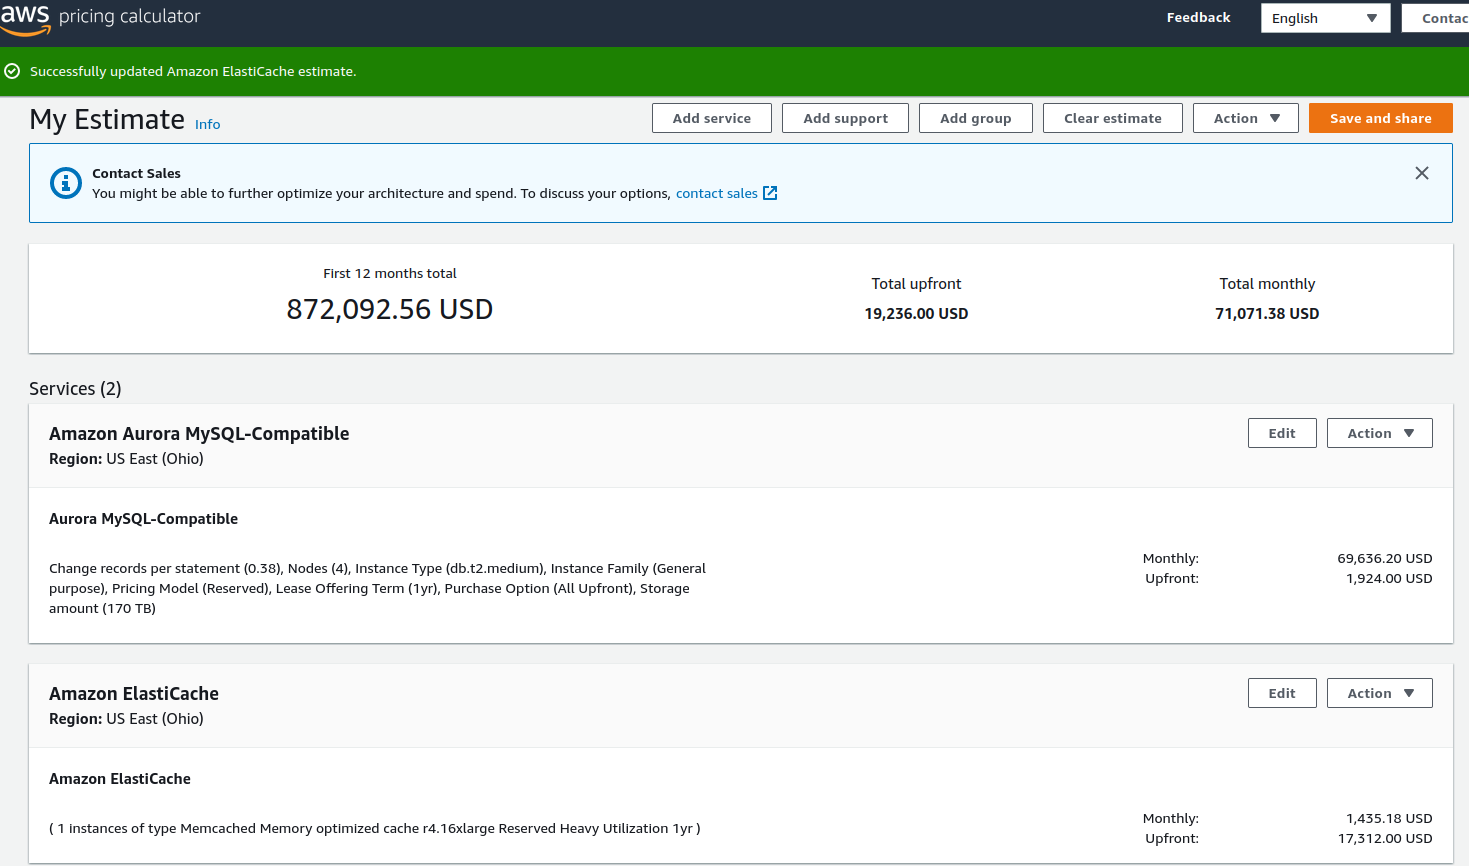
\includegraphics[width=.8\textwidth]{./img/estimate}
  \caption{AWS Estimate}
  \label{fig:estimate}
\end{figure}


This is a real barrier to adoption for emerging BI\&A efforts. Big data is not inexpensive and without demonstrated returns on the investment, most organizations are not going to spend the resources to pursue what is still theoretical advantages.

Even very large organizations are going to focus primarily on more proven technologies rather than pursuing new areas of primary research.

\section{Overcoming the Gap}

Like previous areas of BI\&A, adoption will start with the largest companies when they are presented with supported products from reliable vendors. There will be a typical adoption curve, with some companies seeking an advantage by being an early adopter, and others taking a more ``wait-and-see'' approach. Once the vendors have mastered building and delivering the technology, it will become more of a commodity product and offerings will appear aimed at smaller-to-mid-sized companies. However, the SMC adopters will likely not enjoy the success of social analytics that larger companies will enjoy due to the cost of data storage for truely large data sets.

However, there likely will arise a market for big-data service providers. For example, a company that was performing dynamic social analytics mapping of a metro area could reasonably expect to sell the results of that analysis to any number of marketing firms, thus permitting an economically reasonable ecosystem to arise around the technology, with the resulting analysis provided as a purchased service.
